\documentclass[tikz,border=3mm]{standalone}
\begin{document}
	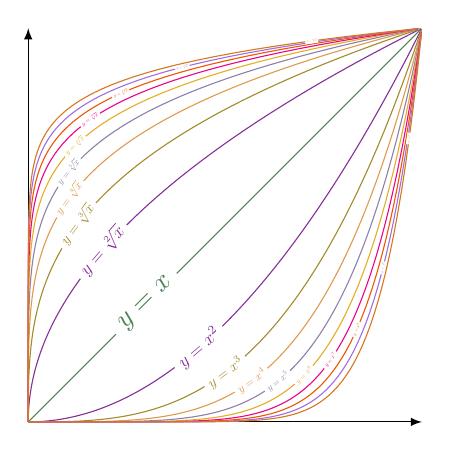
\begin{tikzpicture}[scale=5]
		\draw[latex-latex] (1,0)-|(0,1);
		\foreach \i in {1,...,10}{
			\pgfmathsetmacro{\R}{rnd}
			\pgfmathsetmacro{\G}{rnd}
			\pgfmathsetmacro{\B}{rnd}
			\definecolor{mau}{rgb}{\R,\G,\B}
			\draw[samples=100,mau]
			plot[domain=0:1] ({(\x)^\i},\x)
			plot[domain=0:1] (\x,{(\x)^\i});
			\ifnum\i>1\def\a{0.3}\def\da{0.001}\def\n{15}
			\path[mau] (\a+\i/\n,{(\a+\i/\n)^\i})--(\a+\da+\i/\n,{(\a+\da+\i/\n)^\i}) node[pos=1,sloped,scale=0.8^\i,fill=white]{$y=x^{\i}$}
			({(\a+\i/15)^\i},\a+\i/\n)--({(\a+\da+\i/\n)^\i},\a+\da+\i/\n) node[pos=1,sloped,scale=0.8^\i,fill=white]{$y=\sqrt[\i]{x}$}
			\else
			\path[mau] (0.3,0.3) node[rotate=45,fill=white]{$y=x$};
			\fi
			;
		}
	\end{tikzpicture}
\end{document}